\documentclass[12pt,a4paper]{ctexart}
\usepackage[margin=2.2cm]{geometry}
\usepackage{graphicx}
\usepackage{booktabs}
\usepackage{amsmath}
\usepackage{float}
\usepackage{hyperref}
\usepackage{xcolor}
\usepackage{listings}

\lstset{
	language=C,
	basicstyle=\ttfamily\small,
	keywordstyle=\color{blue!70!black},
	commentstyle=\color{green!40!black},
	stringstyle=\color{orange!60!black},
	showstringspaces=false,
	breaklines=true,
	frame=single,
	tabsize=4
}

% ===== 实验信息 =====
\newcommand{\reporttitle}{实验三：LR(0) 项目集规范族构建}
\newcommand{\subtask}{闭包、Goto 与 LR(0) 冲突检测}
\newcommand{\authname}{姓名}
\newcommand{\authid}{学号}
% =====================

\title{\reporttitle}
\author{\authname：\underline{李祥熙} \quad \authid：\underline{2234412799}}
\date{\today}

\begin{document}
\maketitle

\section{实验目的}
本实验的目标如下：
\begin{itemize}
	\item 构建给定文法的 LR(0) 项目集规范族，理解闭包与 Goto 的构造过程。
	\item 输出每个状态的项目集与状态转移关系，形成规范族的完整视图。
	\item 检测移进-归约与归约-归约冲突，判断文法是否为 LR(0)。
\end{itemize}

\section{实验过程}
\subsection{实验环境}
\begin{itemize}
	\item 操作系统：Linux
	\item 编程语言：C（C11）
	\item 编译工具：GCC
	\item 其他工具：LaTeX（ctexart），VS Code
\end{itemize}

\subsection{数据集与输入形式}
本实验的输入为文法规则文件 \texttt{grammar.txt}，支持扩展巴科斯范式（\texttt{|}）与空产生式（\texttt{epsilon}）。
同一文件中包含多个示例文法，便于在同一程序中复用读取逻辑。

\textbf{输入文法：}

\lstinputlisting[language=]{../grammar.txt}

\textbf{说明：}该文件包含三个文法片段，分别是表达式文法、赋值语句文法与经典 \texttt{CC} 文法。
程序默认将第一条产生式左侧视作起始符号（本次为 \texttt{E}），也支持在命令行指定起始符号。

\subsection{实现步骤}
\begin{enumerate}
	\item 解析输入文法，分离非终结符与终结符，构建产生式集合并自动增广文法。
	\item 基于增广起始项目生成初始项目集，计算闭包（Closure）。
	\item 对每个项目集与符号计算 Goto，生成新的项目集并编号。
	\item 输出项目集、状态转移图，并检测 LR(0) 冲突。
\end{enumerate}

\section{实验内容}
\subsection{任务一：文法解析与增广}
程序支持形如 \texttt{E -> E + T | T} 的规则，并允许多行输入。
读取阶段先收集非终结符集合，再解析右部符号序列，最后自动构造增广产生式 \texttt{S' -> S}。

\subsection{任务二：闭包与 Goto 构造}
闭包过程：对于形如 $A \rightarrow \alpha \cdot B \beta$ 的项目，加入 \texttt{B} 的全部产生式项目 $B \rightarrow \cdot \gamma$，直到不再变化。
Goto 过程：对项目集中点后为某符号的项目进行移点，形成新项目集并计算其闭包。

以下代码片段展示了闭包与 Goto 的核心实现：
\begin{lstlisting}
static void
closure (ItemSet *set, const Production *prods, const int *nonterm_first,
				 const int *nonterm_count, const int *symbol_is_nonterm)
{
	int changed = 1;
	while (changed)
		{
			changed = 0;
			for (int i = 0; i < set->count; ++i)
				{
					Item it = set->items[i];
					const Production *p = &prods[it.prod];
					if (it.dot >= p->rhs_len)
						{
							continue;
						}
					int sym = p->rhs[it.dot];
					if (!symbol_is_nonterm[sym])
						{
							continue;
						}
					int nt_index = sym;
					int start = nonterm_first[nt_index];
					int cnt = nonterm_count[nt_index];
					if (start < 0 || cnt <= 0)
						{
							continue;
						}
					for (int k = 0; k < cnt; ++k)
						{
							Item new_item;
							new_item.prod = start + k;
							new_item.dot = 0;
							if (!itemset_contains (set, &new_item))
								{
									itemset_add (set, &new_item);
									changed = 1;
								}
						}
				}
		}
}

static void
goto_set (const ItemSet *src, int symbol, ItemSet *dst,
					const Production *prods, int prod_count, const int *nonterm_first,
					const int *nonterm_count, int nonterm_total,
					const int *symbol_is_nonterm)
{
	dst->count = 0;
	for (int i = 0; i < src->count; ++i)
		{
			Item it = src->items[i];
			const Production *p = &prods[it.prod];
			if (it.dot < p->rhs_len && p->rhs[it.dot] == symbol)
				{
					Item moved;
					moved.prod = it.prod;
					moved.dot = it.dot + 1;
					itemset_add (dst, &moved);
				}
		}
	(void)prod_count;
	(void)nonterm_total;
	closure (dst, prods, nonterm_first, nonterm_count, symbol_is_nonterm);
	itemset_sort (dst);
}
\end{lstlisting}

\textbf{说明：}闭包函数按“能扩展就扩展”的方式迭代加入新项目；Goto 函数负责点向右移动并调用闭包，形成完整的新状态。

\section{实验结果}
\subsection{任务一结果：程序运行截图}
\begin{figure}[H]
\centering
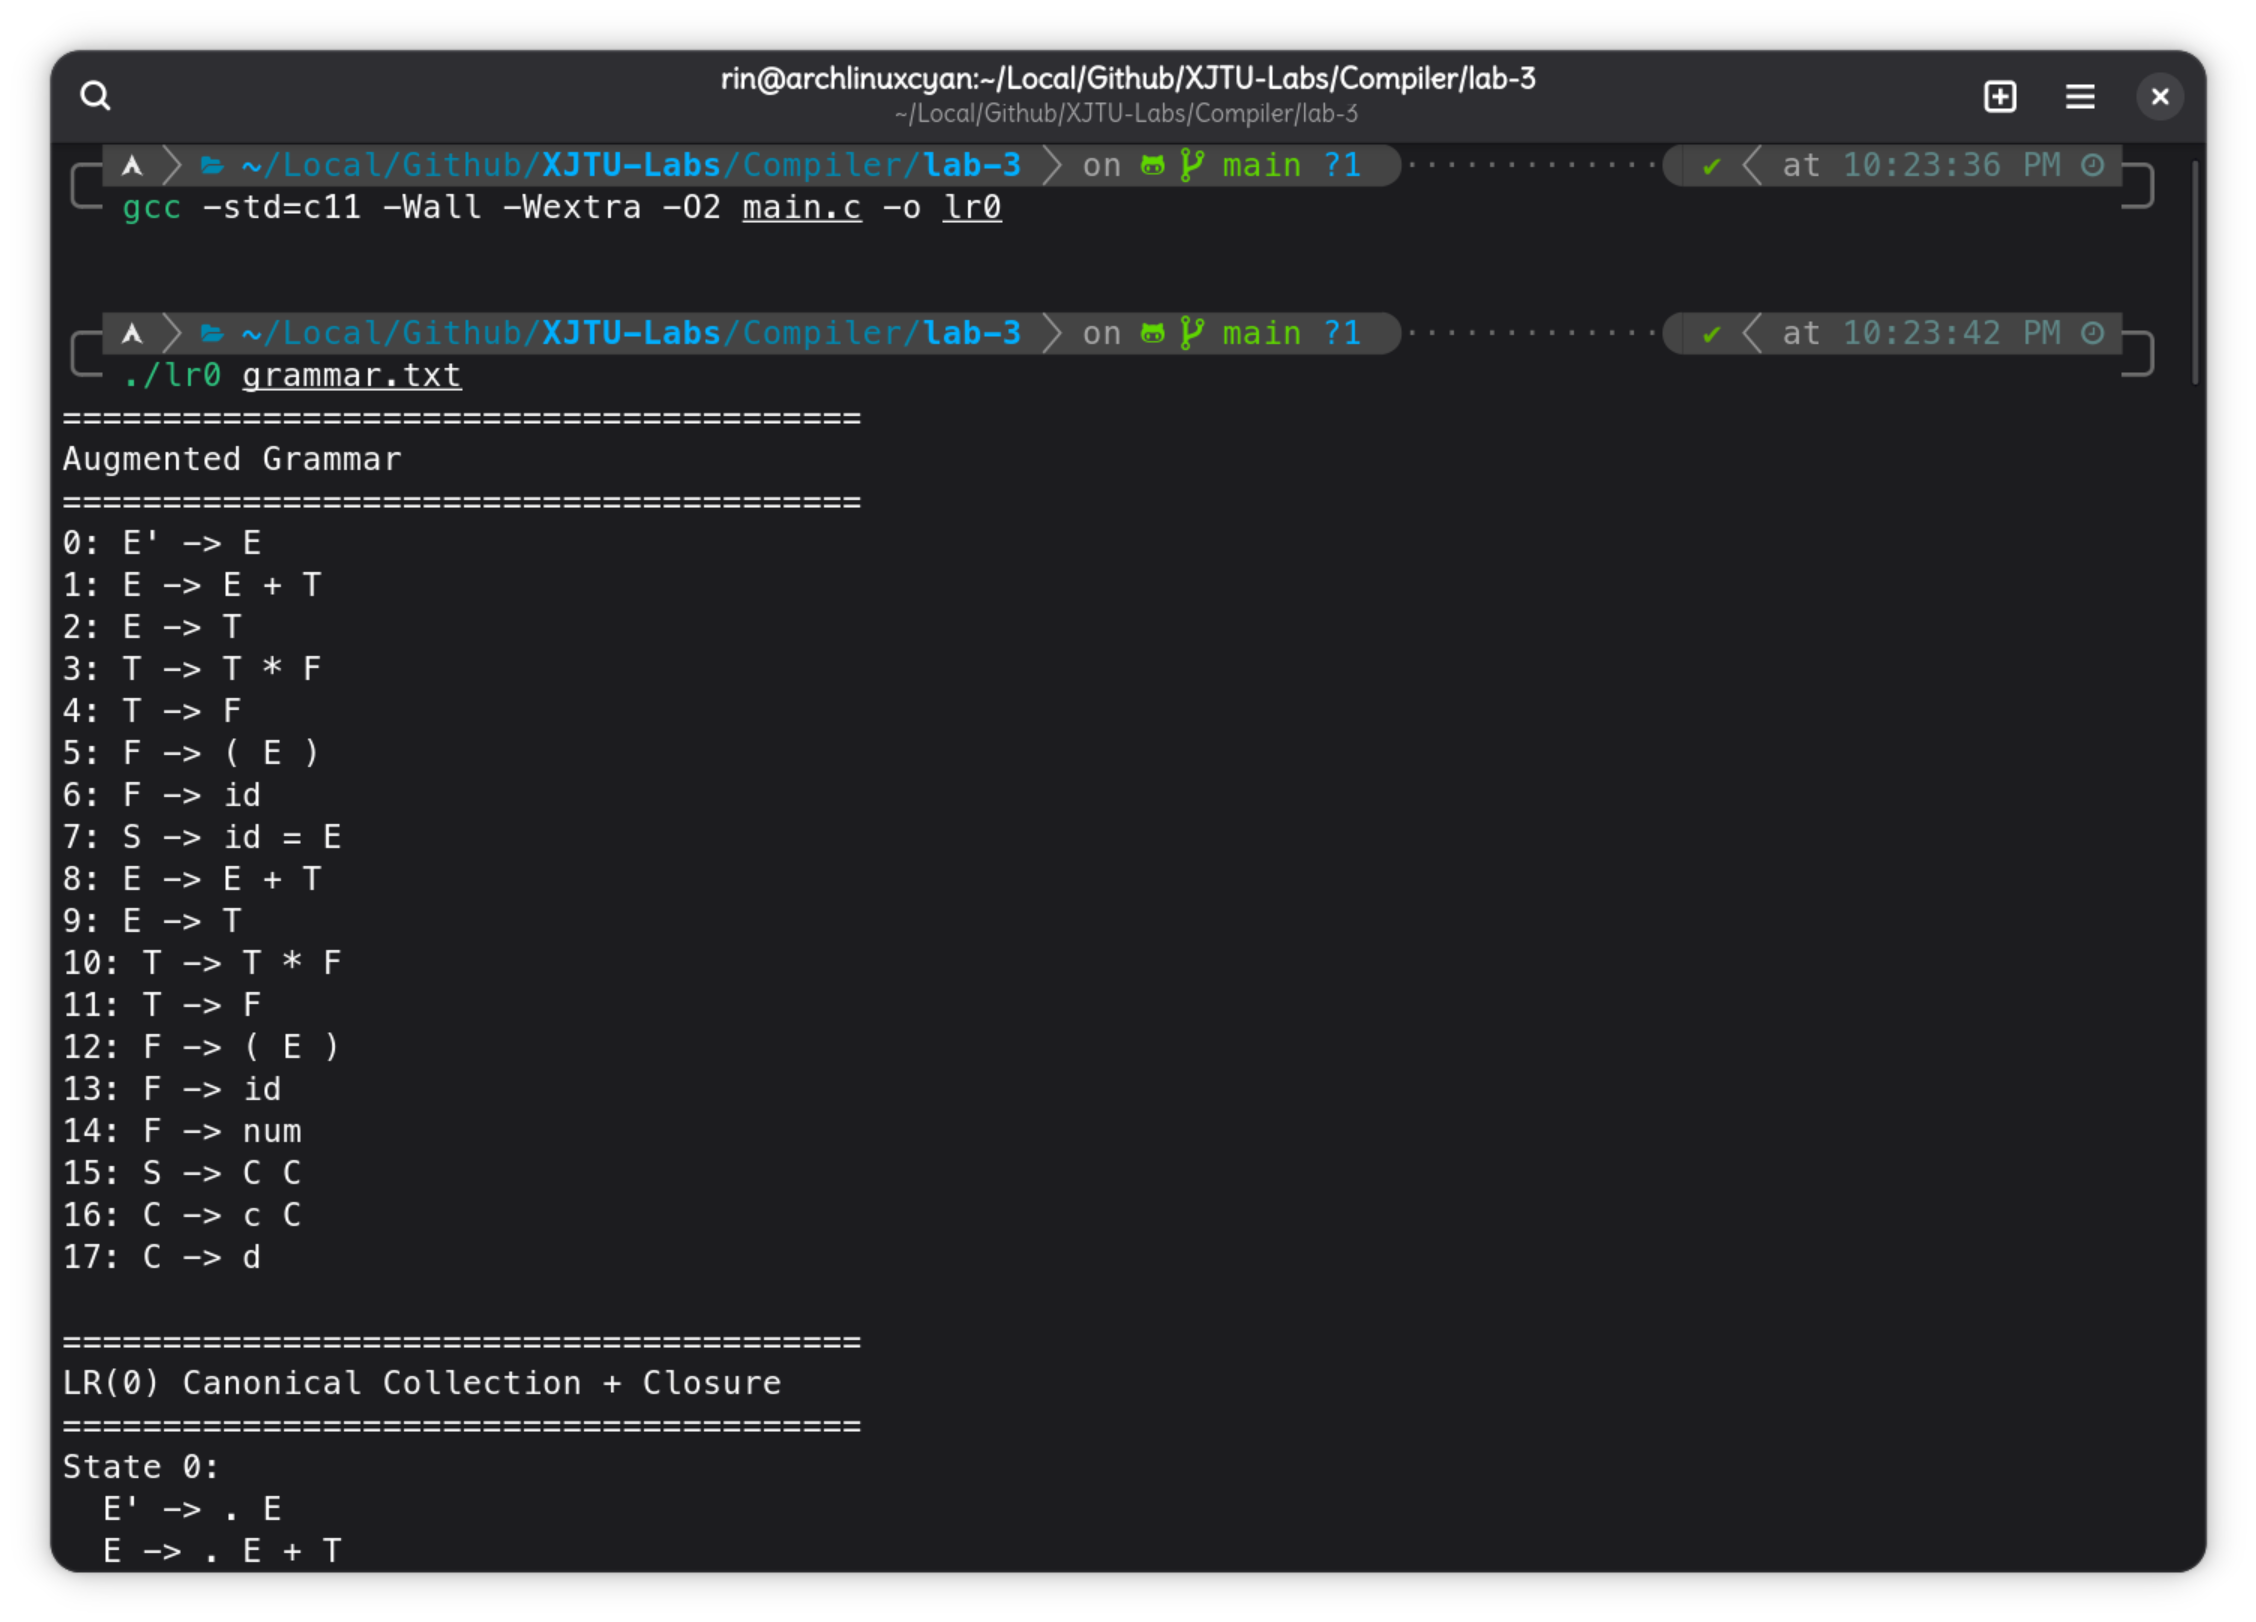
\includegraphics[width=0.95\textwidth]{images/compile_and_run.png}
\caption{程序编译与运行截图}
\label{fig:run}
\end{figure}

结果分析：
\begin{itemize}
	\item 程序能够成功读取文法并输出增广文法与项目集状态。
	\item 屏幕输出与预期格式一致，便于对照状态编号与转移。
\end{itemize}

\subsection{任务二结果：项目集与冲突检测输出}

\begin{lstlisting}
{
========================================
Augmented Grammar
========================================
0: E' -> E
1: E -> E + T
2: E -> T
3: T -> T * F
4: T -> F
5: F -> ( E )
6: F -> id
7: S -> id = E
8: E -> E + T
9: E -> T
10: T -> T * F
11: T -> F
12: F -> ( E )
13: F -> id
14: F -> num
15: S -> C C
16: C -> c C
17: C -> d

========================================
LR(0) Canonical Collection + Closure
========================================
State 0:
  E' -> . E
  E -> . E + T
  E -> . T
  T -> . T * F
  T -> . F
  F -> . ( E )
  F -> . id
  S -> . id = E
  E -> . E + T
  E -> . T
Kernel: E' -> . E

State 1:
  E' -> E .
  E -> E . + T
  E -> E . + T
Kernel: E' -> E ., E -> E . + T, E -> E . + T

State 2:
  E -> T .
  T -> T . * F
  E -> T .
Kernel: E -> T ., T -> T . * F, E -> T .

State 3:
  T -> F .
Kernel: T -> F .

State 4:
  E -> . E + T
  E -> . T
  T -> . T * F
  T -> . F
  F -> . ( E )
  F -> ( . E )
  F -> . id
  S -> . id = E
  E -> . E + T
  E -> . T
Kernel: F -> ( . E )

State 5:
  F -> id .
  S -> id . = E
Kernel: F -> id ., S -> id . = E

State 6:
  E -> . E + T
  E -> E + . T
  E -> . T
  T -> . T * F
  T -> . F
  F -> . ( E )
  F -> . id
  S -> . id = E
  E -> . E + T
  E -> E + . T
  E -> . T
Kernel: E -> E + . T, E -> E + . T

State 7:
  E -> . E + T
  E -> . T
  T -> . T * F
  T -> T * . F
  T -> . F
  F -> . ( E )
  F -> . id
  S -> . id = E
  E -> . E + T
  E -> . T
Kernel: T -> T * . F

State 8:
  E -> E . + T
  F -> ( E . )
  E -> E . + T
Kernel: E -> E . + T, F -> ( E . ), E -> E . + T

State 9:
  E -> . E + T
  E -> . T
  T -> . T * F
  T -> . F
  F -> . ( E )
  F -> . id
  S -> . id = E
  S -> id = . E
  E -> . E + T
  E -> . T
Kernel: S -> id = . E

State 10:
  E -> E . + T
  E -> E . + T
Kernel: E -> E . + T, E -> E . + T

State 11:
  E -> E + T .
  E -> T .
  T -> T . * F
  E -> E + T .
  E -> T .
Kernel: E -> E + T ., E -> T ., T -> T . * F, E -> E + T ., E -> T .

State 12:
  T -> T * F .
  T -> F .
Kernel: T -> T * F ., T -> F .

State 13:
  F -> ( E ) .
Kernel: F -> ( E ) .

State 14:
  E -> E . + T
  S -> id = E .
  E -> E . + T
Kernel: E -> E . + T, S -> id = E ., E -> E . + T

========================================
State Transition Graph
========================================
0 --E--> 1
0 --T--> 2
0 --F--> 3
0 --(--> 4
0 --id--> 5
1 --+--> 6
2 --*--> 7
4 --E--> 8
4 --T--> 2
4 --F--> 3
4 --(--> 4
4 --id--> 5
5 --=--> 9
6 --E--> 10
6 --T--> 11
6 --F--> 3
6 --(--> 4
6 --id--> 5
7 --E--> 10
7 --T--> 2
7 --F--> 12
7 --(--> 4
7 --id--> 5
8 --+--> 6
8 --)--> 13
9 --E--> 14
9 --T--> 2
9 --F--> 3
9 --(--> 4
9 --id--> 5
10 --+--> 6
11 --*--> 7
14 --+--> 6
========================================
LR(0) Conflict Check
========================================
State 2: reduce-reduce conflict
State 2: shift-reduce conflict
State 5: shift-reduce conflict
State 11: reduce-reduce conflict
State 11: shift-reduce conflict
State 12: reduce-reduce conflict
State 14: shift-reduce conflict
Grammar has conflicts, not LR(0).
}
\end{lstlisting}

\textbf{说明：}输出包含四部分：增广文法、LR(0) 规范族、状态转移图与冲突检测结论。
从结果可以看出该文法存在多处移进-归约与归约-归约冲突，因此整体不是 LR(0) 文法。
这也符合将多个示例文法合并在同一文件中时的预期现象。

\section{总结}
本实验完成了 LR(0) 项目集规范族构建与冲突检测：
\begin{itemize}
	\item 实现了文法解析与自动增广，支持扩展巴科斯范式输入。
	\item 输出了项目集闭包与状态转移图，能够直接观察规范族结构。
	\item 通过冲突检查给出 LR(0) 判定结论，为后续 SLR(1) 表构造奠定基础。
\end{itemize}

\section*{附录：实验源代码}
\subsection*{A.1 主要源码：main.c}

\begin{lstlisting}
#include <ctype.h>
#include <stdio.h>
#include <stdlib.h>
#include <string.h>
#ifdef __unix__
#include <unistd.h>
#endif

#define MAX_LINE 1024
#define MAX_LINES 512
#define MAX_PRODS 512
#define MAX_RHS 32
#define MAX_SYMBOLS 256
#define MAX_STATES 256
#define MAX_ITEMS 4096
#define MAX_NAME 64

typedef struct
{
  int lhs;
  int rhs[MAX_RHS];
  int rhs_len;
} Production;

typedef struct
{
  int prod;
  int dot;
} Item;

typedef struct
{
  Item items[MAX_ITEMS];
  int count;
} ItemSet;

static void
trim (char *s)
{
  size_t n = strlen (s);
  while (n > 0 && (s[n - 1] == '\n' || s[n - 1] == '\r'))
    {
      s[n - 1] = '\0';
      --n;
    }
  size_t i = 0;
  while (s[i] && isspace ((unsigned char)s[i]))
    {
      ++i;
    }
  if (i > 0)
    {
      memmove (s, s + i, strlen (s + i) + 1);
    }
  n = strlen (s);
  while (n > 0 && isspace ((unsigned char)s[n - 1]))
    {
      s[n - 1] = '\0';
      --n;
    }
}

static int
is_blank (const char *s)
{
  while (*s)
    {
      if (!isspace ((unsigned char)*s))
        {
          return 0;
        }
      ++s;
    }
  return 1;
}

static int
starts_with (const char *s, const char *prefix)
{
  return strncmp (s, prefix, strlen (prefix)) == 0;
}

static int
find_arrow (const char *s)
{
  const char *p = strstr (s, "->");
  if (!p)
    {
      return -1;
    }
  return (int)(p - s);
}

static int
name_index (char names[][MAX_NAME], int count, const char *name)
{
  for (int i = 0; i < count; ++i)
    {
      if (strcmp (names[i], name) == 0)
        {
          return i;
        }
    }
  return -1;
}

static int
add_name (char names[][MAX_NAME], int *count, const char *name)
{
  int idx = name_index (names, *count, name);
  if (idx >= 0)
    {
      return idx;
    }
  if (*count >= MAX_SYMBOLS)
    {
      return -1;
    }
  strncpy (names[*count], name, MAX_NAME - 1);
  names[*count][MAX_NAME - 1] = '\0';
  (*count)++;
  return (*count) - 1;
}

static int
is_nonterminal (char nonterms[][MAX_NAME], int nonterm_count, const char *s)
{
  return name_index (nonterms, nonterm_count, s) >= 0;
}

static int
item_equal (const Item *a, const Item *b)
{
  return a->prod == b->prod && a->dot == b->dot;
}

static int
itemset_contains (const ItemSet *set, const Item *it)
{
  for (int i = 0; i < set->count; ++i)
    {
      if (item_equal (&set->items[i], it))
        {
          return 1;
        }
    }
  return 0;
}

static void
itemset_add (ItemSet *set, const Item *it)
{
  if (!itemset_contains (set, it))
    {
      if (set->count < MAX_ITEMS)
        {
          set->items[set->count++] = *it;
        }
    }
}

static int
item_cmp (const void *a, const void *b)
{
  const Item *ia = (const Item *)a;
  const Item *ib = (const Item *)b;
  if (ia->prod != ib->prod)
    {
      return ia->prod - ib->prod;
    }
  return ia->dot - ib->dot;
}

static void
itemset_sort (ItemSet *set)
{
  qsort (set->items, (size_t)set->count, sizeof (Item), item_cmp);
}

static int
itemset_equal (const ItemSet *a, const ItemSet *b)
{
  if (a->count != b->count)
    {
      return 0;
    }
  for (int i = 0; i < a->count; ++i)
    {
      if (!item_equal (&a->items[i], &b->items[i]))
        {
          return 0;
        }
    }
  return 1;
}

static void
closure (ItemSet *set, const Production *prods, const int *nonterm_first,
         const int *nonterm_count, const int *symbol_is_nonterm)
{
  int changed = 1;
  while (changed)
    {
      changed = 0;
      for (int i = 0; i < set->count; ++i)
        {
          Item it = set->items[i];
          const Production *p = &prods[it.prod];
          if (it.dot >= p->rhs_len)
            {
              continue;
            }
          int sym = p->rhs[it.dot];
          if (!symbol_is_nonterm[sym])
            {
              continue;
            }
          int nt_index = sym;
          int start = nonterm_first[nt_index];
          int cnt = nonterm_count[nt_index];
          if (start < 0 || cnt <= 0)
            {
              continue;
            }
          for (int k = 0; k < cnt; ++k)
            {
              Item new_item;
              new_item.prod = start + k;
              new_item.dot = 0;
              if (!itemset_contains (set, &new_item))
                {
                  itemset_add (set, &new_item);
                  changed = 1;
                }
            }
        }
    }
}

static void
goto_set (const ItemSet *src, int symbol, ItemSet *dst,
          const Production *prods, int prod_count, const int *nonterm_first,
          const int *nonterm_count, int nonterm_total,
          const int *symbol_is_nonterm)
{
  dst->count = 0;
  for (int i = 0; i < src->count; ++i)
    {
      Item it = src->items[i];
      const Production *p = &prods[it.prod];
      if (it.dot < p->rhs_len && p->rhs[it.dot] == symbol)
        {
          Item moved;
          moved.prod = it.prod;
          moved.dot = it.dot + 1;
          itemset_add (dst, &moved);
        }
    }
  (void)prod_count;
  (void)nonterm_total;
  closure (dst, prods, nonterm_first, nonterm_count, symbol_is_nonterm);
  itemset_sort (dst);
}

static void
print_production (const Production *p, char symbols[][MAX_NAME])
{
  printf ("%s ->", symbols[p->lhs]);
  if (p->rhs_len == 0)
    {
      printf (" epsilon");
    }
  else
    {
      for (int i = 0; i < p->rhs_len; ++i)
        {
          printf (" %s", symbols[p->rhs[i]]);
        }
    }
}

static void
print_item (const Item *it, const Production *prods, char symbols[][MAX_NAME])
{
  const Production *p = &prods[it->prod];
  printf ("%s ->", symbols[p->lhs]);
  for (int i = 0; i < p->rhs_len; ++i)
    {
      if (i == it->dot)
        {
          printf (" .");
        }
      printf (" %s", symbols[p->rhs[i]]);
    }
  if (it->dot == p->rhs_len)
    {
      printf (" .");
    }
}

static void
collect_kernel (const ItemSet *set, ItemSet *kernel)
{
  kernel->count = 0;
  for (int i = 0; i < set->count; ++i)
    {
      Item it = set->items[i];
      if (it.dot > 0 || it.prod == 0)
        {
          itemset_add (kernel, &it);
        }
    }
  itemset_sort (kernel);
}

static int
parse_grammar_lines (char lines[][MAX_LINE], int line_count,
                     char nonterms[][MAX_NAME], int *nonterm_count,
                     char symbols[][MAX_NAME], int *symbol_count,
                     int *start_symbol, Production *prods, int *prod_count)
{
  *nonterm_count = 0;
  *symbol_count = 0;
  *prod_count = 0;

  for (int i = 0; i < line_count; ++i)
    {
      char buf[MAX_LINE];
      strncpy (buf, lines[i], sizeof (buf) - 1);
      buf[sizeof (buf) - 1] = '\0';
      trim (buf);
      if (is_blank (buf) || starts_with (buf, "#") || starts_with (buf, "//"))
        {
          continue;
        }
      int arrow = find_arrow (buf);
      if (arrow < 0)
        {
          return 0;
        }
      buf[arrow] = '\0';
      buf[arrow + 1] = '\0';
      char lhs[MAX_NAME];
      strncpy (lhs, buf, sizeof (lhs) - 1);
      lhs[sizeof (lhs) - 1] = '\0';
      trim (lhs);
      if (lhs[0] == '\0')
        {
          return 0;
        }
      add_name (nonterms, nonterm_count, lhs);
    }

  if (*nonterm_count == 0)
    {
      return 0;
    }

  for (int i = 0; i < *nonterm_count; ++i)
    {
      add_name (symbols, symbol_count, nonterms[i]);
    }

  *start_symbol = 0;

  for (int i = 0; i < line_count; ++i)
    {
      char buf[MAX_LINE];
      strncpy (buf, lines[i], sizeof (buf) - 1);
      buf[sizeof (buf) - 1] = '\0';
      trim (buf);
      if (is_blank (buf) || starts_with (buf, "#") || starts_with (buf, "//"))
        {
          continue;
        }

      int arrow = find_arrow (buf);
      if (arrow < 0)
        {
          return 0;
        }

      buf[arrow] = '\0';
      char rhs_part[MAX_LINE];
      strncpy (rhs_part, buf + arrow + 2, sizeof (rhs_part) - 1);
      rhs_part[sizeof (rhs_part) - 1] = '\0';

      char lhs[MAX_NAME];
      strncpy (lhs, buf, sizeof (lhs) - 1);
      lhs[sizeof (lhs) - 1] = '\0';
      trim (lhs);
      if (lhs[0] == '\0')
        {
          return 0;
        }

      int lhs_sym = name_index (symbols, *symbol_count, lhs);
      if (lhs_sym < 0)
        {
          return 0;
        }

      char *alt = rhs_part;
      while (alt)
        {
          char *bar = strchr (alt, '|');
          if (bar)
            {
              *bar = '\0';
            }
          char alt_buf[MAX_LINE];
          strncpy (alt_buf, alt, sizeof (alt_buf) - 1);
          alt_buf[sizeof (alt_buf) - 1] = '\0';
          trim (alt_buf);

          Production p;
          p.lhs = lhs_sym;
          p.rhs_len = 0;

          if (alt_buf[0] == '\0' || strcmp (alt_buf, "epsilon") == 0
              || strcmp (alt_buf, "eps") == 0)
            {
              p.rhs_len = 0;
            }
          else
            {
              char *tok = strtok (alt_buf, " \t");
              while (tok)
                {
                  int sym;
                  if (is_nonterminal (nonterms, *nonterm_count, tok))
                    {
                      sym = name_index (symbols, *symbol_count, tok);
                    }
                  else
                    {
                      sym = name_index (symbols, *symbol_count, tok);
                      if (sym < 0)
                        {
                          sym = add_name (symbols, symbol_count, tok);
                        }
                    }
                  if (sym < 0)
                    {
                      return 0;
                    }
                  if (p.rhs_len >= MAX_RHS)
                    {
                      return 0;
                    }
                  p.rhs[p.rhs_len++] = sym;
                  tok = strtok (NULL, " \t");
                }
            }

          if (*prod_count >= MAX_PRODS)
            {
              return 0;
            }
          prods[(*prod_count)++] = p;

          if (bar)
            {
              alt = bar + 1;
            }
          else
            {
              alt = NULL;
            }
        }
    }

  return 1;
}

int
main (int argc, char **argv)
{
  char (*lines)[MAX_LINE] = malloc (sizeof (*lines) * MAX_LINES);
  if (!lines)
    {
      fprintf (stderr, "Out of memory.\n");
      return 1;
    }
  int line_count = 0;

  FILE *fp = stdin;
  if (argc >= 2)
    {
      fp = fopen (argv[1], "r");
      if (!fp)
        {
          fprintf (stderr, "Cannot open file: %s\n", argv[1]);
          return 1;
        }
    }

  while (line_count < MAX_LINES && fgets (lines[line_count], MAX_LINE, fp))
    {
      trim (lines[line_count]);
      if (!is_blank (lines[line_count]))
        {
          line_count++;
        }
    }

  if (fp != stdin)
    {
      fclose (fp);
    }

  if (line_count == 0)
    {
      fprintf (stderr, "No grammar rules provided.\n");
      return 1;
    }

  char (*nonterms)[MAX_NAME] = malloc (sizeof (*nonterms) * MAX_SYMBOLS);
  char (*symbols)[MAX_NAME] = malloc (sizeof (*symbols) * MAX_SYMBOLS);
  if (!nonterms || !symbols)
    {
      fprintf (stderr, "Out of memory.\n");
      return 1;
    }
  int nonterm_count = 0;
  int symbol_count = 0;
  int start_symbol = 0;
  Production *prods = malloc (sizeof (*prods) * MAX_PRODS);
  if (!prods)
    {
      fprintf (stderr, "Out of memory.\n");
      return 1;
    }
  int prod_count = 0;

  if (!parse_grammar_lines (lines, line_count, nonterms, &nonterm_count,
                            symbols, &symbol_count, &start_symbol, prods,
                            &prod_count))
    {
      fprintf (stderr,
               "Failed to parse grammar. Ensure lines like: E -> E + T | T\n");
      return 1;
    }

  if (argc >= 3)
    {
      int idx = name_index (symbols, symbol_count, argv[2]);
      if (idx < 0)
        {
          fprintf (stderr, "Start symbol '%s' not found in grammar.\n",
                   argv[2]);
          return 1;
        }
      start_symbol = idx;
    }

  char aug_name[MAX_NAME];
  snprintf (aug_name, sizeof (aug_name), "%s'", symbols[start_symbol]);
  if (name_index (symbols, symbol_count, aug_name) >= 0)
    {
      snprintf (aug_name, sizeof (aug_name), "%s0", symbols[start_symbol]);
    }

  int aug_sym = add_name (symbols, &symbol_count, aug_name);
  if (aug_sym < 0)
    {
      fprintf (stderr, "Too many symbols.\n");
      return 1;
    }

  Production aug;
  aug.lhs = aug_sym;
  aug.rhs_len = 1;
  aug.rhs[0] = start_symbol;

  Production all_prods[MAX_PRODS];
  int all_prod_count = 0;
  all_prods[all_prod_count++] = aug;
  for (int i = 0; i < prod_count; ++i)
    {
      all_prods[all_prod_count++] = prods[i];
    }

  int *symbol_is_nonterm = calloc (MAX_SYMBOLS, sizeof (int));
  if (!symbol_is_nonterm)
    {
      fprintf (stderr, "Out of memory.\n");
      return 1;
    }
  for (int i = 0; i < nonterm_count; ++i)
    {
      int idx = name_index (symbols, symbol_count, nonterms[i]);
      if (idx >= 0)
        {
          symbol_is_nonterm[idx] = 1;
        }
    }
  symbol_is_nonterm[aug_sym] = 1;

  int *nonterm_first = malloc (sizeof (int) * MAX_SYMBOLS);
  int *nonterm_prod_count = malloc (sizeof (int) * MAX_SYMBOLS);
  if (!nonterm_first || !nonterm_prod_count)
    {
      fprintf (stderr, "Out of memory.\n");
      return 1;
    }
  for (int i = 0; i < MAX_SYMBOLS; ++i)
    {
      nonterm_first[i] = -1;
      nonterm_prod_count[i] = 0;
    }

  for (int i = 0; i < all_prod_count; ++i)
    {
      int lhs = all_prods[i].lhs;
      if (nonterm_first[lhs] < 0)
        {
          nonterm_first[lhs] = i;
        }
      nonterm_prod_count[lhs]++;
    }

  for (int i = 0; i < symbol_count; ++i)
    {
      if (symbol_is_nonterm[i] && nonterm_prod_count[i] == 0)
        {
          fprintf (stderr, "Nonterminal '%s' has no productions.\n",
                   symbols[i]);
          return 1;
        }
    }

  printf ("========================================\n");
  printf ("Augmented Grammar\n");
  printf ("========================================\n");
  for (int i = 0; i < all_prod_count; ++i)
    {
      printf ("%d: ", i);
      print_production (&all_prods[i], symbols);
      printf ("\n");
    }

  ItemSet *states = calloc (MAX_STATES, sizeof (ItemSet));
  if (!states)
    {
      fprintf (stderr, "Out of memory.\n");
      return 1;
    }
  int state_count = 0;
  int (*transitions)[MAX_SYMBOLS]
      = malloc (sizeof (*transitions) * MAX_STATES);
  if (!transitions)
    {
      fprintf (stderr, "Out of memory.\n");
      return 1;
    }
  for (int i = 0; i < MAX_STATES; ++i)
    {
      for (int j = 0; j < MAX_SYMBOLS; ++j)
        {
          transitions[i][j] = -1;
        }
    }

  ItemSet start_set;
  start_set.count = 0;
  Item start_item;
  start_item.prod = 0;
  start_item.dot = 0;
  itemset_add (&start_set, &start_item);

  closure (&start_set, all_prods, nonterm_first, nonterm_prod_count,
           symbol_is_nonterm);
  itemset_sort (&start_set);
  states[state_count++] = start_set;

  for (int i = 0; i < state_count; ++i)
    {
      for (int sym = 0; sym < symbol_count; ++sym)
        {
          ItemSet next;
          goto_set (&states[i], sym, &next, all_prods, all_prod_count,
                    nonterm_first, nonterm_prod_count, symbol_count,
                    symbol_is_nonterm);
          if (next.count == 0)
            {
              continue;
            }
          int existing = -1;
          for (int k = 0; k < state_count; ++k)
            {
              if (itemset_equal (&states[k], &next))
                {
                  existing = k;
                  break;
                }
            }
          if (existing < 0)
            {
              if (state_count >= MAX_STATES)
                {
                  fprintf (stderr, "Too many states.\n");
                  return 1;
                }
              states[state_count] = next;
              existing = state_count;
              state_count++;
            }
          transitions[i][sym] = existing;
        }
    }

  printf ("\n========================================\n");
  printf ("LR(0) Canonical Collection + Closure\n");
  printf ("========================================\n");

  for (int i = 0; i < state_count; ++i)
    {
      printf ("State %d:\n", i);
      for (int j = 0; j < states[i].count; ++j)
        {
          printf ("  ");
          print_item (&states[i].items[j], all_prods, symbols);
          printf ("\n");
        }
      ItemSet kernel;
      collect_kernel (&states[i], &kernel);
      printf ("Kernel: ");
      for (int k = 0; k < kernel.count; ++k)
        {
          if (k > 0)
            {
              printf (", ");
            }
          print_item (&kernel.items[k], all_prods, symbols);
        }
      printf ("\n\n");
    }

  printf ("========================================\n");
  printf ("State Transition Graph\n");
  printf ("========================================\n");
  for (int i = 0; i < state_count; ++i)
    {
      for (int sym = 0; sym < symbol_count; ++sym)
        {
          int to = transitions[i][sym];
          if (to >= 0)
            {
              printf ("%d --%s--> %d\n", i, symbols[sym], to);
            }
        }
    }

  printf ("========================================\n");
  printf ("LR(0) Conflict Check\n");
  printf ("========================================\n");

  int has_conflict = 0;
  for (int i = 0; i < state_count; ++i)
    {
      int shift = 0;
      int reduce_count = 0;
      for (int j = 0; j < states[i].count; ++j)
        {
          Item it = states[i].items[j];
          Production *p = &all_prods[it.prod];
          if (it.dot < p->rhs_len)
            {
              int sym = p->rhs[it.dot];
              if (!symbol_is_nonterm[sym])
                {
                  shift = 1;
                }
            }
          else
            {
              if (it.prod != 0)
                {
                  reduce_count++;
                }
            }
        }

      if (reduce_count > 1)
        {
          printf ("State %d: reduce-reduce conflict\n", i);
          has_conflict = 1;
        }
      if (reduce_count >= 1 && shift)
        {
          printf ("State %d: shift-reduce conflict\n", i);
          has_conflict = 1;
        }
    }

  if (has_conflict)
    {
      printf ("Grammar has conflicts, not LR(0).\n");
    }
  else
    {
      printf ("No conflicts detected. Grammar is LR(0).\n");
    }

  return 0;
}
\end{lstlisting}


\subsection*{A.2 运行命令}
\begin{verbatim}
gcc -std=c11 -Wall -Wextra -O2 main.c -o lr0

# 默认起始符号为第一条产生式左侧（本次为 E）
./lr0 grammar.txt

# 显式指定起始符号
./lr0 grammar.txt E
\end{verbatim}

\end{document}
